\newpage
\section{QR decomposition}
\label{sec:QR}



%%%%%%%%%%%%%%%%%%%%%%%%%%%%%%%%%%%%%%%%%%%%%%%%%%%%%%%%%%%%%%%%%%%%%%%%%%%%%%%%%%%%%%%%%%%%%%%%%%%%
\subsection{Theory}
%%%%%%%%%%%%%%%%%%%%%%%%%%%%%%%%%%%%%%%%%%%%%%%%%%%%%%%%%%%%%%%%%%%%%%%%%%%%%%%%%%%%%%%%%%%%%%%%%%%%



%%%%%%%%%%%%%%%%%%%%%%%%%%%%%%%%%%%%%%%%%%%%%%%%%%

\subsubsection{Orthogonal matrices}
\label{sec:orthogonalMatrices}

Orthogonal matrices represent either reflections or rotations and fulfill by definition the equations:

\begin{align}
\label{eq:definitionOrthogonal0}
\mathbf{Q}\mathbf{Q}^T = \mathbf{I}\\
\label{eq:definitionOrthogonal1}
\mathbf{Q}^T\mathbf{Q} = \mathbf{I}
\end{align}
%
Therefore, the transposed of an orthogonal matrix is also its inverse:
\begin{align}
\label{eq:orthogonalInverse}
\mathbf{Q}^T = \mathbf{Q}^{-1}
\end{align}
%
Another useful property of orthogonal matrices is, that they preserve the length of a vector during matrix-vector multiplication:
\begin{align}
\label{eq:orthogonalPreserveLength}
\norm{\mathbf{Qx}}= \norm{\mathbf{y}}
\end{align}
%
Additionally, the dot product of two vectors remains the same after multiplication with an orthogonal matrix:

\begin{align}
\dotProduct{\mathbf{Q}\mathbf{x}}{\mathbf{Q}\mathbf{y}} &= \dotProduct{\mathbf{x}}{\mathbf{y}}
\end{align}
%
Consequently, the angle between both vectors does not change.



%%%%%%%%%%%%%%%%%%%%%%%%%%%%%%%%%%%%%%%%%%%%%%%%%%

\subsubsection{Solving linear systems with QR decomposition}

The QR decomposition decomposes a matrix $\mathbf{A}$ into an orthogonal matrix $\mathbf{Q}$ and an upper triangular matrix $\mathbf{R}$. 
Solving linear systems with QR decomposition is pretty much straight forward:
\begin{align}
\mathbf{A}\mathbf{x} &= \mathbf{r}\\
\mathbf{QR}\mathbf{x} &= \mathbf{r}
\end{align}
%
The product $\mathbf{R}\mathbf{x}$ is substituted by the vector $\mathbf{y}$:

\begin{align}
\mathbf{Qy} &= \mathbf{r}
\end{align}
%
Since $\mathbf{Q}$ is orthogonal, it follows:

\begin{align}
\mathbf{y} &= \mathbf{Q}^{-1}\mathbf{r}\\
\label{eq:qrSolveIntermediate}
\mathbf{y} &= \mathbf{Q}^T\mathbf{r}
\end{align}
%
The system's solution $\mathbf{x}$ is now obtained by simple backward substitution (see \cref{sec:backwardSubstitution}) because of $\mathbf{R}$ being an upper triangular matrix.
\begin{align}
\label{eq:qrSolveResult}
\mathbf{R}\mathbf{x} = \mathbf{y}
\end{align}
%
The QR decomposition itself can be calculated with different techniques, namely the Gram-Schmidt process, Givens rotations and Householder reflections.
In this document, Householder reflections are used to calculate the decomposition.
In contrast to the Gram-Schmidt approach, they produce numerically stable results.
Their disadvantage of not being parallelizable is not relevant, since systems which benefit of parallelization are usually to large for a real-time engine.
Givens rotations are much more complex regarding the implementation without offering any real benefit within the scope of small linear systems. 
 


%%%%%%%%%%%%%%%%%%%%%%%%%%%%%%%%%%%%%%%%%%%%%%%%%%

\subsubsection{Householder reflections}

A householder reflection is a reflection at a plane or hyperplane that contains the origin of the coordinate system.
Because the origin is by definition part of the reflection plane, only the plane's normal $\mathbf{w}$ is needed to describe it mathematically.
An example is shown in \cref{fig:housholderReflection}.
The Householder matrix $\mathbf{H}$, which performs the reflection during multiplication, is calculated as follows:


\begin{figure}
	\centering
	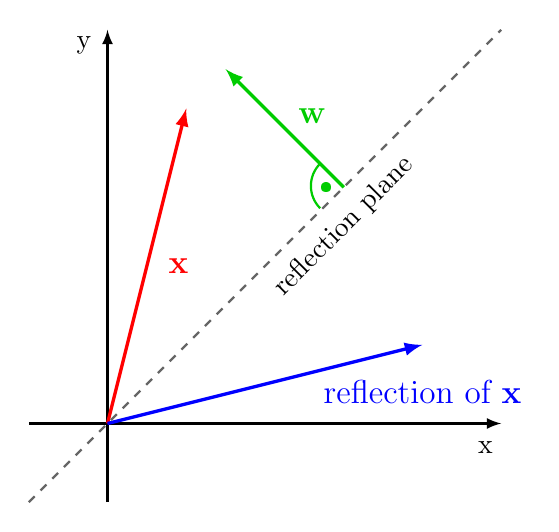
\begin{tikzpicture}
	\draw[color=black,-latex,thick] (-1,0)--(5,0);
	\draw[color=black,-latex,thick] (0,-1)--(0,5);
	\draw[color=red,-latex,very thick] (0,0)--(1,4);
	\draw[color=blue,-latex,very thick] (0,0)--(4,1);
	\draw[color={black!20!green},-latex,very thick] (3,3)--(1.5,4.5);
	\draw[color={black!20!green}, thick] (2.7,3.3) arc (135:225:0.4);
	\node[color={black!20!green}] at (2.78,2.98) {\textbullet};
	\draw[color={black!60!white},dashed,thick] (-1,-1)--(5,5);
	\node[] at (4.8,-0.3) {x};
	\node[] at (-0.3,4.8) {y};
	\node[color=red] at (0.9,2) {\large{$\mathbf{x}$}};
	\node[color=blue] at (4,0.4) {\large{reflection of $\mathbf{x}$}};
	\node[color={black!20!green}] at (2.6,3.9) {\large{$\mathbf{w}$}};
	\node[rotate=45] at (3,2.5) {reflection plane};
	\end{tikzpicture}
	\caption{Householder reflection}
	\label{fig:housholderReflection}
\end{figure}


\begin{align}
\label{eq:householderGeneral}
\mathbf{H} = \mathbf{I} - \frac{2}{\mathbf{w}^T\mathbf{w}}\mathbf{w}\mathbf{w}^T
\end{align}
%
$\mathbf{w}^T\mathbf{w}$ is the scalar product. With $\mathbf{v}$ being the unit normal of the reflection plane

\begin{align}
	\mathbf{v} = \frac{1}{\norm{\mathbf{w}}}\mathbf{w}
\end{align}
%
\cref{eq:householderGeneral} simplifies to:

\begin{align}
\label{eq:householderUnitLength}
\mathbf{H} = \mathbf{I} - 2\mathbf{v}\mathbf{v}^T
\end{align}
%
The Householder matrix $\mathbf{H}$ has some useful properties.
First, it is orthogonal (\cref{sec:orthogonalMatrices}).
Additionally, it is also symmetric, hence:

\begin{align}
\label{eq:householderSymmetric}
\mathbf{H} = \mathbf{H}^T
\end{align}
%
Combining \cref{eq:householderSymmetric} with \cref{eq:orthogonalInverse} yields:

\begin{align}
\label{eq:householderInverse}
\mathbf{H} = \mathbf{H}^{-1}
\end{align}
%
So a Householder matrix is its own inverse.
Furthermore, abusing the Householder matrix's special structure, the product with another vector or matrix can be computed more efficiently than the standard matrix-vector product or matrix-matrix product:

\begin{align}
\nonumber
\mathbf{H} \mathbf{x}
&= 
\pth{\mathbf{I} - 2\mathbf{v}\mathbf{v}^T}\mathbf{x}
\\&= 
\nonumber
\mathbf{I}\mathbf{x} - 2\mathbf{v}\mathbf{v}^T\mathbf{x}
\\&= 
\label{eq:householderEfficientMatrixVector}
\mathbf{x} - 2\pth{\mathbf{v}^T\mathbf{x}}\mathbf{v}
\end{align}
%
Note that $\mathbf{v}^T\mathbf{x}$ is the scalar product.
Instead of the quadratic complexity of the standard matrix-vector product, \cref{eq:householderEfficientMatrixVector} is only of linear complexity.
For matrix-matrix multiplication, the approach is similar and results in quadratic complexity instead of cubic:

\begin{align}
\label{eq:householderEfficientMatrixMatrix}
\mathbf{H} \mathbf{A}
=
\mathbf{A} - 2\mathbf{v}\pth{\mathbf{v}^T\mathbf{A}}
\end{align}
%
$\mathbf{v}^T\mathbf{A}$ is a row vector that contains the scalar products of $\mathbf{v}$ and each column of $\mathbf{A}$



%%%%%%%%%%%%%%%%%%%%%%%%%%%%%%%%%%%%%%%%%%%%%%%%%%

\subsubsection{Calculation of a specific Householder reflection}
\label{sec:householderCalculateSpecificReflection}

Consider the case, that two vectors $\mathbf{x}$ and $\mathbf{y}$ of arbitrary length are known and the reflection, which transforms $\mathbf{x}$ in a way that it points into the same direction as $\mathbf{y}$ (without scaling it), should be determined.
The equation that describes this problem is:

\begin{align}
\label{eq:housholderCalculateReflection}
\mathbf{H} \mathbf{x} = \lambda \mathbf{y}
\end{align}
%
Since orthogonal matrices preserve a vectors length (see \cref{eq:orthogonalPreserveLength}) it follows:

\begin{align}
\label{eq:housholderCalculateReflectionLambda}
\lambda = \pm \frac{\norm{\mathbf{x}}}{\norm{\mathbf{y}}}
\end{align}
%
Therefore, $\lambda$ is the length ratio of the vectors $\mathbf{x}$ and $\mathbf{y}$.
Taking a look at \cref{fig:housholderCalculateReflection} reveals that the difference between the vectors $\mathbf{x}$ and $\mathbf{Hx}$ is orthogonal to the reflection plane.
Hence, the required normal can be calculated with:

\begin{align}
\label{eq:housholderCalculateReflectionNormal}
\mathbf{w} &= \mathbf{x} - \lambda \mathbf{y}
\end{align}
%
The unit length normal is obtained by:
%
\begin{align}
\label{eq:housholderCalculateReflectionUnitNormal}
\mathbf{v} &= \frac{1}{\norm{\mathbf{x} - \lambda \mathbf{y}}}\pth{\mathbf{x} - \lambda \mathbf{y}}
\end{align}


\begin{figure}
\centering
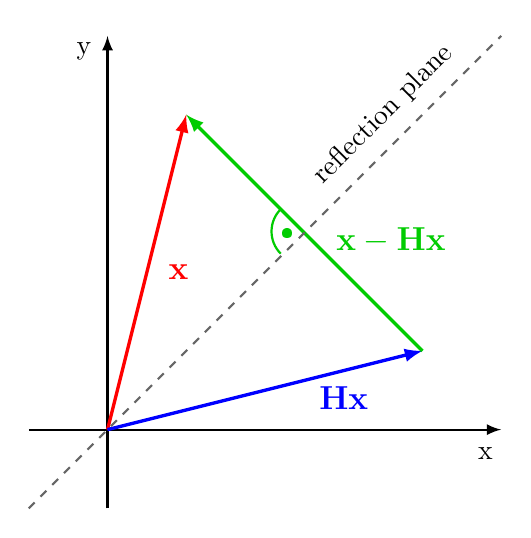
\begin{tikzpicture}
\draw[color=black,-latex,thick] (-1,0)--(5,0);
\draw[color=black,-latex,thick] (0,-1)--(0,5);
\draw[color=red,-latex,very thick] (0,0)--(1,4);
\draw[color=blue,-latex,very thick] (0,0)--(4,1);
\draw[color={black!20!green},-latex,very thick] (4,1)--(1,4);
\draw[color={black!20!green}, thick] (2.2,2.8) arc (135:225:0.4);
\node[color={black!20!green}] at (2.28,2.48) {\textbullet};
\draw[color={black!60!white},dashed,thick] (-1,-1)--(5,5);
\node[] at (4.8,-0.3) {x};
\node[] at (-0.3,4.8) {y};
\node[color=red] at (0.9,2) {\large{$\mathbf{x}$}};
\node[color=blue] at (3,0.4) {\large{$\mathbf{Hx}$}};
\node[color={black!20!green}] at (3.6,2.4) {\large{$\mathbf{x-Hx}$}};
\node[rotate=45] at (3.5,4) {reflection plane};
\end{tikzpicture}
\caption{Difference between original and reflected vector}
\label{fig:housholderCalculateReflection}
\end{figure}



%%%%%%%%%%%%%%%%%%%%%%%%%%%%%%%%%%%%%%%%%%%%%%%%%%

\subsubsection{Calculation of the decomposition}
\label{sec:qrCalculateDecomposition}

The algorithm to calculate the QR decomposition using Householder reflections is rather simple, once the concepts of the previous sections are understood.
A series of Householder reflections is calculated and multiplied with the target matrix, so that each value below the main diagonal becomes 0.
At the end of this process, the upper triangular matrix $\mathbf{R}$ is obtained.
The matrix $\mathbf{Q}$ can be determined by multiplication of all used Householder matrices, but usually, it is not necessary to calculate it explicitly.

The exact procedure is now discussed on an example.
Consider the matrix:

\begin{align*}
\mathbf{A}
=
\begin{bmatrix}
\mathbf{a} & \mathbf{b} & \mathbf{c} & \mathbf{d}
\end{bmatrix}
=
\begin{bmatrix}
a_0&b_0&c_0&d_0\\
a_1&b_1&c_1&d_1\\
a_2&b_2&c_2&d_2\\
a_3&b_3&c_3&d_3
\end{bmatrix}
\end{align*}
%
The algorithm starts by calculating a Householder reflection that turns all values of the first column below the main diagonal into zeros:

\begin{align}
\mathbf{H}\mathbf{A} 
=
\mathbf{\bar{A}}
=
\begin{bmatrix}
\mathbf{\bar{a}} & \mathbf{\bar{b}} & \mathbf{\bar{c}} & \mathbf{\bar{d}}
\end{bmatrix}
=
\begin{bmatrix}
\bar{a}_0&\bar{b}_0&\bar{c}_0&\bar{d}_0\\
0        &\bar{b}_1&\bar{c}_1&\bar{d}_1\\
0        &\bar{b}_2&\bar{c}_2&\bar{d}_2\\
0        &\bar{b}_3&\bar{c}_3&\bar{d}_3
\end{bmatrix}					  
\end{align}
%
Note, that varying numbers of bars above variable names are used to differ between multiple intermediate results.
The necessary first Householder transformation must reflects the column $\mathbf{a}$ of the original matrix $\mathbf{A}$ onto the axis
\begin{align}
\mathbf{e}  
=
\begin{bmatrix}
1\\
0\\
0\\
0
\end{bmatrix}
\end{align}
%
Using \cref{eq:housholderCalculateReflectionUnitNormal} yields

\begin{align}
\mathbf{v} 
&= 
\frac{1}{\norm{\mathbf{a} - \lambda \mathbf{e}}}\pth{\mathbf{a} - \lambda \mathbf{e}}\\
&=
\frac{1}{\norm{\mathbf{a} - \lambda \mathbf{e}}}
\pth{
\begin{bmatrix}
a_0\\
a_1\\
a_2\\
a_3
\end{bmatrix}
-	
\lambda	
\begin{bmatrix}
1\\
0\\
0\\
0
\end{bmatrix}
}\\
\label{eq:qrReflectionVector0StillContainingLambda}
&=
\frac{1}{\norm{\mathbf{a} - \lambda \mathbf{e}}}
\begin{bmatrix}
a_0 - \lambda\\
a_1\\
a_2\\
a_3
\end{bmatrix}
\end{align}
%
Since $\mathbf{e}$ is of unit length, \cref{eq:housholderCalculateReflectionLambda} gives:

\begin{align}
\lambda = \pm \norm{\mathbf{a}}
\end{align}
%
Generally, the sign can be chosen freely, but for numerical reasons one should pick the opposite sign of $a_0$. 
This way the result with the larger magnitude is selected from $a_0 -  \pm \norm{\mathbf{a}}$.
To illustrate why this is necessary, consider the case where $\mathbf{a} = \mathbf{e}$.
Using the same sign yields:

\begin{align}
\mathbf{e} - \norm{\mathbf{e}}\mathbf{e} 
=
\begin{bmatrix}
1 - \norm{\mathbf{e}}\\
0\\
0\\
0
\end{bmatrix}
=
\begin{bmatrix}
0\\
0\\
0\\
0 
\end{bmatrix}
\end{align}
%
and in result:

\begin{align}
\frac{1}{\norm{\mathbf{e} - \norm{\mathbf{e}}\mathbf{e}}} = \frac{1}{\color{red}{\mathbf{0}}}
\end{align}
%
Choosing the opposite sign prevents this from happening unless $\mathbf{a}$ is already of length 0, which would indicate that the matrix is singular.
Combining 


\begin{align}
\lambda = -\textrm{sign}\pth{a_0} \norm{\mathbf{a}}
\end{align}
%
with \cref{eq:qrReflectionVector0StillContainingLambda} yields:



\begin{align}
\mathbf{v} 
&=
\frac{1}{\norm{\mathbf{w}}}\mathbf{w}
\end{align}
%
with:

\begin{align}
\mathbf{w} 
&=
\begin{bmatrix}
a_0 + \textrm{sign}\pth{a_0} \norm{\mathbf{a}}\\
a_1\\
a_2\\
a_3
\end{bmatrix}
\end{align}
%
Now the intermediate matrix $\mathbf{\bar{A}}$ can be determined by calculating $\mathbf{H}$ with \cref{eq:householderUnitLength} and multiplying it with $\mathbf{A}$.
However, the more efficient way is to use \cref{eq:householderEfficientMatrixMatrix}.
Also, keep in mind that the vector $\lambda\mathbf{e}$, which was used to calculate the reflection normal, is equal to the first column $\mathbf{\bar{a}}$ of $\mathbf{\bar{A}}$.
So there is no need to calculate it again.

After obtaining $\mathbf{\bar{A}}$, a second reflection $\mathbf{\bar{H}}$ is calculated which eliminates all values below the main diagonal in the second column:

\begin{align}
\mathbf{\bar{H}}\mathbf{H}\mathbf{A} 
= 
\mathbf{\bar{H}}\mathbf{\bar{A}}
= 
\mathbf{\bar{\bar{A}}}
=
\begin{bmatrix}
\mathbf{\bar{\bar{a}}}&\mathbf{\bar{\bar{b}}}&\mathbf{\bar{\bar{c}}}&\mathbf{\bar{\bar{d}}}
\end{bmatrix}	
=
\begin{bmatrix}
\bar{\bar{a}}_0&\bar{\bar{b}}_0&\bar{\bar{c}}_0&\bar{\bar{d}}_0\\
0              &\bar{\bar{b}}_1&\bar{\bar{c}}_1&\bar{\bar{d}}_1\\
0              &0              &\bar{\bar{c}}_2&\bar{\bar{d}}_2\\
0              &0              &\bar{\bar{c}}_3&\bar{\bar{d}}_3
\end{bmatrix}					  
\end{align}
%
Note that $\mathbf{\bar{H}}$ must be constructed in a way, that it doesn't affect values that lie on the axis $\mathbf{e}$ (first row of $\mathbf{\bar{A}}$).
Otherwise, because of \cref{eq:orthogonalPreserveLength}, one or more values below $\bar{a}_0$ in $\mathbf{\bar{a}}$ will become different from 0 again.
This can only be achieved if the reflection plane contains the axis $\mathbf{e}$.
Hence, the reflection plane's normal $\mathbf{\bar{v}}$ must be orthogonal to $\mathbf{e}$ and has the form: 

\begin{align}
\label{eq:qrReflectionVector1Requirement}
\mathbf{\bar{v}}
= 
\begin{bmatrix}
0\\
\bar{v}_1\\
\bar{v}_2\\
\bar{v}_3
\end{bmatrix}
\end{align}
%
The corresponding Householder matrix $\mathbf{\bar{H}}$ is obtained with \cref{eq:householderUnitLength}:

\begin{align}
\mathbf{\bar{H}}
=
\begin{bmatrix}
1    &0                   &0                   &0                   \\
0    &1-\bar{v}_1\bar{v}_1&  \bar{v}_1\bar{v}_2&  \bar{v}_1\bar{v}_3\\
0    &  \bar{v}_2\bar{v}_1&1-\bar{v}_2\bar{v}_2&  \bar{v}_2\bar{v}_3\\
0    &  \bar{v}_3\bar{v}_1&  \bar{v}_3\bar{v}_2&1-\bar{v}_3\bar{v}_3
\end{bmatrix}					  
\end{align}
%
As can be checked, this matrix doesn't change the first column and row when multiplied with $\mathbf{\bar{A}}$.
However, calculating the components of $\mathbf{\bar{v}}$ gets a bit more complicated.
Using \cref{eq:housholderCalculateReflection} gives:

\begin{align}
\mathbf{\bar{H}} \mathbf{\bar{b}} 
= 
\bar{\lambda} \mathbf{\bar{e}}
= 
\bar{\lambda} 
\begin{bmatrix}
\bar{e}_0\\
\bar{e}_1\\
0\\
0
\end{bmatrix}
=  
\begin{bmatrix}
\bar{\bar{b}}_0\\
\bar{\bar{b}}_1\\
0\\
0
\end{bmatrix}
= 
\mathbf{\bar{\bar{b}}} 
\end{align}
%
The vector $\mathbf{\bar{e}}$ doesn't lie on a coordinate axis, as it was the case during the calculation of the first reflection.
Instead, it lies on a plane spanned by two of the coordinate system's axes.
Because of the constraint that the transformation is not allowed to modify the first component of $\mathbf{\bar{b}}$, the values $\bar{e}_0$ and $\bar{e}_1$ can not be chosen arbitrarily.
However, this constraint also means that:

\begin{align}
\bar{b}_0 = \bar{\bar{b}}_0 = \bar{\lambda}\bar{e}_0
\end{align}
%
Since the difference of $\mathbf{\bar{b}}$ and $\mathbf{\bar{\bar{b}}}$ is a normal of the reflection plane (compare \cref{sec:householderCalculateSpecificReflection}), it follows:

\begin{align}
\mathbf{\bar{w}}
= 
\begin{bmatrix}
\bar{w}_0\\
\bar{w}_1\\
\bar{w}_2\\
\bar{w}_3
\end{bmatrix}
= 
\begin{bmatrix}
\bar{b}_0\\
\bar{b}_1\\
\bar{b}_2\\
\bar{b}_3
\end{bmatrix}
-
\begin{bmatrix}
\bar{\bar{b}}_0\\
\bar{\lambda}\bar{e}_1\\
0\\
0
\end{bmatrix}
=
\begin{bmatrix}
0\\
\bar{b}_1 - \bar{\lambda}\bar{e}_1\\
\bar{b}_2\\
\bar{b}_3
\end{bmatrix}
\end{align}
%
The only remaining unknown value is the product $\bar{\lambda}\bar{e}_1$, respectively $\bar{\bar{b}}_1$.
It can be obtained with the property of orthogonal matrices to preserve a vector's length:

\begin{align}
\norm{\mathbf{\bar{b}}} 
&= 
\norm{\mathbf{\bar{\bar{b}}}}
\\
\sqrt{\bar{b}_0^2 + \bar{b}_1^2 + \bar{b}_2^2 + \bar{b}_3^2}
&=
\sqrt{\bar{\bar{b}}_0^2 + \bar{\bar{b}}_1^2}
\end{align}
%
Because of $\bar{b}_0^2 = \bar{\bar{b}}_0^2$ it follows:

\begin{align}
\bar{\bar{b}}_1^2
&=
\bar{b}_1^2 + \bar{b}_2^2 + \bar{b}_3^2 
\\
\\
\bar{\bar{b}}_1
&=
\pm \sqrt{\bar{b}_1^2 + \bar{b}_2^2 + \bar{b}_3^2}
\\
&= \pm \norm{\mathbf{\dot{\bar{b}}}}
\end{align}
%
The vector $\mathbf{\dot{\bar{b}}}$ is equal to $\mathbf{\bar{b}}$ without its first value.
Therefore, $\mathbf{\bar{w}}$ and $\mathbf{\bar{v}}$ are totally independent of $\bar{b}_0$.
In fact, the non-zero components of $\mathbf{\bar{w}}$ can also be obtained from calculating the first reflection's normal 

\begin{align}
\mathbf{\dot{\bar{w}}}
= 
\begin{bmatrix}
\bar{w}_1\\
\bar{w}_2\\
\bar{w}_3
\end{bmatrix}
\end{align}
%
of the reduced matrix:

\begin{align}
\mathbf{\dot{\bar{A}}}
=
\begin{bmatrix}
\mathbf{\dot{\bar{b}}} & \mathbf{\dot{\bar{c}}} & \mathbf{\dot{\bar{d}}}
\end{bmatrix}
=
\begin{bmatrix}
\bar{b}_1&\bar{c}_1&\bar{d}_1\\
\bar{b}_2&\bar{c}_2&\bar{d}_2\\
\bar{b}_3&\bar{c}_3&\bar{d}_3
\end{bmatrix}					  
\end{align}
%
As previously detected, the transformation $\mathbf{\bar{H}}$ does not affect the first row and column of $\mathbf{\bar{A}}$.
Therefore, all components of $\mathbf{\bar{\bar{A}}}$, that differ from those of $\mathbf{\bar{A}}$, can be determined with the reduced system

\begin{align}
\mathbf{\dot{\bar{H}}}\mathbf{\dot{\bar{A}}}
= 
\mathbf{\dot{\bar{\bar{A}}}}
=
\begin{bmatrix}
\mathbf{\dot{\bar{\bar{b}}}}&\mathbf{\dot{\bar{\bar{c}}}}&\mathbf{\dot{\bar{\bar{d}}}}
\end{bmatrix}	
=
\begin{bmatrix}
\bar{\bar{b}}_1&\bar{\bar{c}}_1&\bar{\bar{d}}_1\\
0              &\bar{\bar{c}}_2&\bar{\bar{d}}_2\\
0              &\bar{\bar{c}}_3&\bar{\bar{d}}_3
\end{bmatrix}					  
\end{align}
%
Like the other matrices, $\mathbf{\dot{\bar{H}}}$ is equal to $\mathbf{\bar{H}}$ without the first row and column.
As a graphical example, \cref{fig:householderReflection3d} shows that a reflection plane containing the x-axis  does not affect the reflected vector's x-values and that the normal can be calculated independently of the x-values from the involved vectors.
%
\begin{figure}
\centering
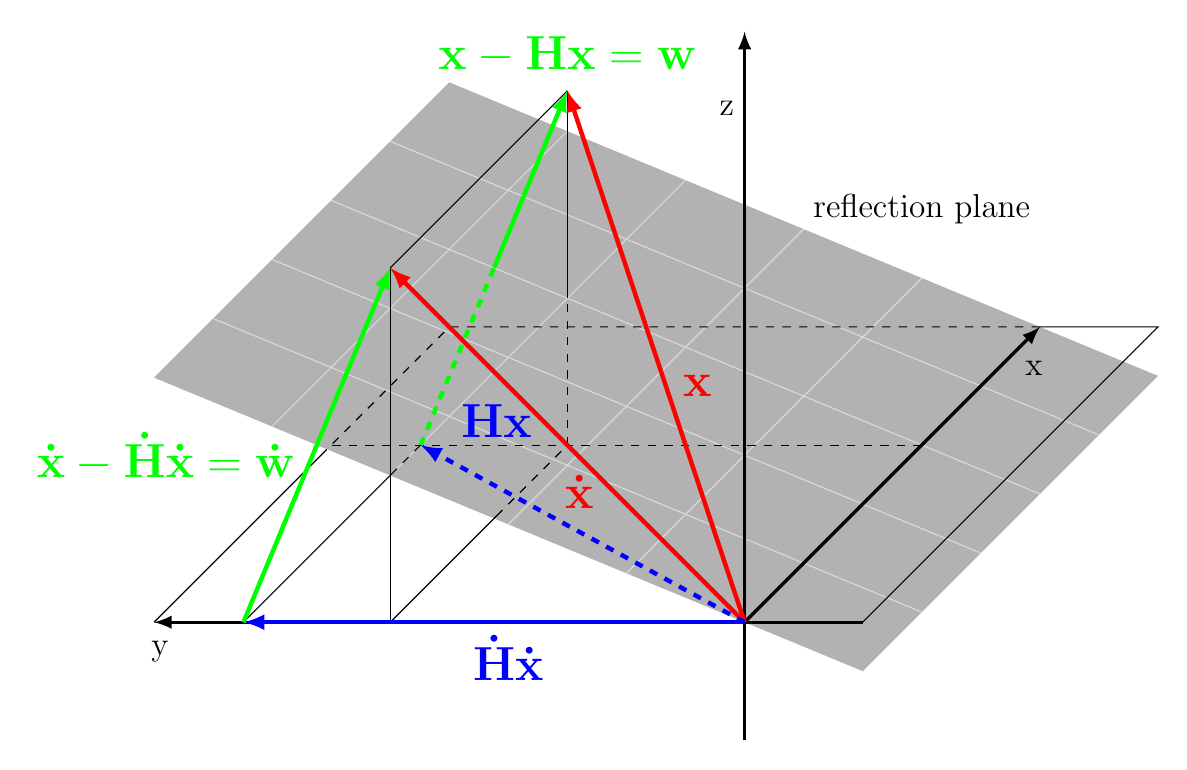
\begin{tikzpicture}
[y  = {(-1cm,0cm)},
x  = {(0.5cm,0.5cm)},
z  = {(0cm,1cm)},
scale = 1.5]
\fill [fill=black!30!white] (0,-1,-0.4142) -- (0,5,2.071) -- (5,5,2.071) -- (5,-1,-0.4142) -- (0,-1,-0.4142);
\draw[color= black!15!white] (1,-1,-0.4142) -- (1,5,2.071);
\draw[color= black!15!white] (2,-1,-0.4142) -- (2,5,2.071);
\draw[color= black!15!white] (3,-1,-0.4142) -- (3,5,2.071);
\draw[color= black!15!white] (4,-1,-0.4142) -- (4,5,2.071);
\draw[color= black!15!white] (0,1, 0.4142) -- (5,1,0.4142);
\draw[color= black!15!white] (0,2, 0.8284) -- (5,2,0.8284);
\draw[color= black!15!white] (0,3, 1.2426) -- (5,3,1.2426);
\draw[color= black!15!white] (0,4, 1.6568) -- (5,4,1.6568);

\draw[-latex, very thick] (0,0,0) -- (5,0,0);
\draw[-latex,  very thick] (0,-1,0) -- (0,5,0);
\draw[-latex, very thick] (0,0,-1) -- (0,0,5);
\draw[] (0,-1,0) -- (5,-1,0) -- (5,0,0);
\draw[dashed] (5,0,0) -- (5,5,0) -- (2.9,5,0);
\draw[] (2.9,5,0) -- (0,5,0);

\draw[] (0,3,3) -- (3,3,3);
\draw[] (0,4.243,0) -- (2.5,4.243,0);
\draw[dashed] (2.5,4.243,0) -- (3,4.243,0);
\draw[dashed] (3,0,0) -- (3,5,0);
\draw[] (0,3,0) -- (0,3,3);
\draw[dashed] (3,3,0) -- (3,3,1.243);
\draw[] (3,3,1.243) -- (3,3,3);
\draw[] (0,3,0) -- (1.8,3,0);
\draw[dashed] (1.8,3,0) -- (3,3,0);


\draw[color=red,-latex, ultra thick] (0,0,0) -- (0,3,3);
\draw[color=blue,-latex, ultra thick] (0,0,0) -- (0,4.243,0);
\draw[color=green, -latex, ultra thick] (0,4.243,0) -- (0,3,3);

\draw[color=red,-latex, ultra thick] (0,0,0) -- (3,3,3);
\draw[color=blue,-latex, dashed, ultra thick] (0,0,0) -- (3,4.243,0);
\draw[color=green, dashed, ultra thick] (3,4.243,0) -- (3,3.6215,1.5);
\draw[color=green, -latex, ultra thick] (3,3.6215,1.5) -- (3,3,3);

\node[] at (4.3,-0.3,0) {\large{x}};
\node[] at (-0.5,4.7,0) {\large{y}};
\node[] at (-0.3,0,4.5) {\large{z}};

\node[] at (5,1,1) {\large{reflection plane}};
\node[color=blue] at (3,3.6,0.2) {\LARGE{$\mathbf{Hx}$}};
\node[color=red] at (1,0.9,1.5) {\LARGE{$\mathbf{x}$}};
\node[color=green] at (3,3,3.3) {\LARGE{$\mathbf{x-Hx =w}$}};

\node[color=blue] at (0,2,-0.3) {\LARGE{$\mathbf{\dot{H}\dot{x}}$}};
\node[color=red] at (0,1.4,1.1) {\LARGE{$\mathbf{\dot{x}}$}};
\node[color=green] at (0,4.9,1.4) {\LARGE{$\mathbf{\dot{x}-\dot{H}\dot{x}=\dot{w}}$}};
\end{tikzpicture}
\caption{Comparison of reflections on a reflection plane containing the x-axis. Dashed lines are covered by the reflection plane.}
\label{fig:householderReflection3d}
\end{figure}
%
The same procedure using reduced systems can be utilized to calculate all following reflections. Hence, the last necessary calculations to obtain 

\begin{align}
\mathbf{R}
= 
\mathbf{\bar{\bar{H}}}\mathbf{\bar{H}}\mathbf{H}\mathbf{A} 
= 
\mathbf{\bar{\bar{H}}}\mathbf{\bar{H}}\mathbf{\bar{A}}
= 
\mathbf{\bar{\bar{H}}}\mathbf{\bar{\bar{A}}}
=
\begin{bmatrix}
\mathbf{\bar{\bar{\bar{a}}}}&\mathbf{\bar{\bar{\bar{b}}}}&\mathbf{\bar{\bar{\bar{c}}}}&\mathbf{\bar{\bar{\bar{d}}}}
\end{bmatrix}	
=
\begin{bmatrix}
\bar{\bar{a}}_0&\bar{\bar{b}}_0&\bar{\bar{c}}_0&\bar{\bar{d}}_0\\
0              &\bar{\bar{b}}_1&\bar{\bar{c}}_1&\bar{\bar{d}}_1\\
0              &0              &\bar{\bar{c}}_2&\bar{\bar{d}}_2\\
0              &0              &\bar{\bar{c}}_3&\bar{\bar{d}}_3
\end{bmatrix}					  
\end{align}
%
can be done using the reduced system:

\begin{align}
\mathbf{\ddot{R}}
= 
\mathbf{\ddot{\bar{\bar{H}}}}\mathbf{\ddot{\bar{\bar{A}}}}
=
\mathbf{\ddot{\bar{\bar{H}}}}
\begin{bmatrix}
\bar{\bar{c}}_2&\bar{\bar{d}}_2\\
\bar{\bar{c}}_3&\bar{\bar{d}}_3
\end{bmatrix}	
=
\begin{bmatrix}
\bar{\bar{\bar{c}}}_2&\bar{\bar{\bar{d}}}_2\\
\bar{\bar{\bar{c}}}_3&\bar{\bar{\bar{d}}}_3
\end{bmatrix}					  
\end{align}
%
Now that $\mathbf{R}$ and all necessary reflections are known, $\mathbf{Q}$ can be determined as follows:

\begin{align}
\mathbf{R} &= \mathbf{\bar{\bar{H}}}\mathbf{\bar{H}}\mathbf{H}\mathbf{A} = \mathbf{Q}^T\mathbf{A}
\\
\\
\mathbf{Q}^T &= \mathbf{\bar{\bar{H}}}\mathbf{\bar{H}}\mathbf{H}\\
\nonumber
\mathbf{Q}   &= \pth{\mathbf{\bar{\bar{H}}}\mathbf{\bar{H}}\mathbf{H}}^T\\
\nonumber
&= \mathbf{H}^T\mathbf{\bar{H}}^T\mathbf{\bar{\bar{H}}}^T\\
&= \mathbf{H}\mathbf{\bar{H}}\mathbf{\bar{\bar{H}}}
\end{align}
%
However, calculating $\mathbf{Q}$ is usually expensive and not necessary. Instead, the reflection normals $\mathbf{v}$, $\mathbf{\bar{v}}$ and $\mathbf{\bar{\bar{v}}}$ are stored and used during the solution process, taking advantage of the effective matrix-vector and matrix-matrix products (\cref{eq:householderEfficientMatrixMatrix,eq:householderEfficientMatrixVector}).
So instead of using \cref{eq:qrSolveIntermediate}, the intermediate result $\mathbf{y}$ of \cref{eq:qrSolveIntermediate} is calculated with:

\begin{align}
\mathbf{y} &= \mathbf{\bar{\bar{H}}}\mathbf{\bar{H}}\mathbf{H}\mathbf{r}
\end{align}
%
Subsequently, the system's solution can be calculated with \cref{eq:qrSolveResult}.


%%%%%%%%%%%%%%%%%%%%%%%%%%%%%%%%%%%%%%%%%%%%%%%%%%

\subsubsection{Algorithm summary}

This section is just a short summary of the algorithm presented in the previous sections.
They should be read first.

For an arbitrary matrix $\mathbf{A}$ of size $N \times N$ calculate:

\begin{align}
\label{eq:qrReflectionUnitNormal}
\mathbf{v} 
&=
\frac{1}{\norm{\mathbf{w}}}\mathbf{w}
\end{align}
%
with 

\begin{align}
\label{eq:qrReflectionNormal}
\mathbf{w} = 
\begin{bmatrix}
a_{00} + \textrm{sign}\pth{a_{00}} \norm{\mathbf{a}_1}\\
a_{10}\\
\vdots\\
a_{\pth{N-1}0}
\end{bmatrix}
\end{align}
%
The vector $\mathbf{a}_1$ is the first column of $\mathbf{A}$. 
Use \cref{eq:householderEfficientMatrixMatrix} to obtain the result of

\begin{align}
\mathbf{H}_1 \mathbf{A} = \mathbf{A}_1
\end{align}
%
without calculating $\mathbf{H}_1$ explicitly.
Remove the first column and row of $\mathbf{A}_1$ and repeat this procedure with the reduced system until the upper triangular matrix $\mathbf{R}$ is obtained.
This will need $N-1$ Householder reflections.
Store the reflection normals $\mathbf{v}_1$ to $\mathbf{v}_{N-1}$ and the matrix $\mathbf{R}$ as QR factorization of $\mathbf{A}$.
To solve the system $\mathbf{A}\mathbf{x}=\mathbf{r}$, calculate the result of

\begin{align}
\mathbf{y} &= \mathbf{Q}^T\mathbf{r}\\
\mathbf{y} &= \mathbf{H}_{N-1} \hdots \mathbf{H}_{2}\mathbf{H}_{1}\mathbf{r}
\end{align}
%
using the vectors $\mathbf{v}_1$ to $\mathbf{v}_{N-1}$ and \cref{eq:householderEfficientMatrixVector}.
Finally, use backward substitution to obtain the systems result $\mathbf{x}$ from 

\begin{align}
\mathbf{R}\mathbf{x} &= \mathbf{y}
\end{align}




%%%%%%%%%%%%%%%%%%%%%%%%%%%%%%%%%%%%%%%%%%%%%%%%%%

\subsubsection{Rectangular matrices}

\draftNote{Start section}



%%%%%%%%%%%%%%%%%%%%%%%%%%%%%%%%%%%%%%%%%%%%%%%%%%%%%%%%%%%%%%%%%%%%%%%%%%%%%%%%%%%%%%%%%%%%%%%%%%%%
\subsection{Optimizations}
%%%%%%%%%%%%%%%%%%%%%%%%%%%%%%%%%%%%%%%%%%%%%%%%%%%%%%%%%%%%%%%%%%%%%%%%%%%%%%%%%%%%%%%%%%%%%%%%%%%%
\label{sec:qrOptimizations}



%%%%%%%%%%%%%%%%%%%%%%%%%%%%%%%%%%%%%%%%%%%%%%%%%%

\subsubsection{Calculation of vector norms}
\label{sec:qrOptimizationsVectorNorms}

During the calculation of each reflection's unit normal $\mathbf{v}$, two vector norms need to be calculated.
Both vectors only differ in a single value.
Therefore, it is beneficial to calculate the squared sum of all shared values and use it to calculate both norms efficiently.

To illustrate this, have a look at the \cref{eq:qrReflectionNormal,eq:qrReflectionUnitNormal}.
In the vectors $\mathbf{a}_1$ and $\mathbf{v}$ share the values $a_{10}$ to $a_{(N-1)0}$.
With the sum 

\begin{align}
s =  \pth{a_{10}}^2  + \pth{a_{20}}^2 + \hdots + \pth{a_{(N-1)0}}^2  
\end{align}
%
the norms can be calculated as follows:

\begin{align}
\norm{\mathbf{a}_1} &= \sqrt{\pth{a_{00}}^2 + s}\\
\norm{\mathbf{w}} &= \sqrt{\pth{a_{00} + \textrm{sign}\pth{a_{00}} \norm{\mathbf{a}_1}}^2 + s}
\end{align}



%%%%%%%%%%%%%%%%%%%%%%%%%%%%%%%%%%%%%%%%%%%%%%%%%%

\subsection{Calculation of intermediate matrix}
\label{sec:qrOptimizationsFirstColumn}

It was already mentioned in \cref{sec:qrCalculateDecomposition} and is repeated here, that it is not necessary to perform any calculation to obtain the first column of the new intermediate (sub)matrix when applying the current decomposition steps reflection.

In the first column of the new matrix, only the first component differs from zero.
Since orthogonal matrices preserve vector lengths, it must be equal to the column's norm before the transformation.
This value was already determined during the calculation of the reflection normal.



%%%%%%%%%%%%%%%%%%%%%%%%%%%%%%%%%%%%%%%%%%%%%%%%%%

\subsubsection{Compact factorization data storage}
\label{sec:qrOptimizationsCompactData}

At this point, it should be mentioned that storing the calculated reflection's unit normals instead of calculating Q explicitly is already an optimization regarding performance and memory consumption.
Storing all necessary unit normals column by column produces an $N \times \pth{N-1}$ matrix $\mathbf{V}$ with all values above the main diagonal being zeros.

\begin{align}
\mathbf{V} = 
\begin{bmatrix}
v_0 & 0         & 0\\
v_1 & \bar{v}_1 & 0\\
v_2 & \bar{v}_2 & \bar{\bar{v}}_2 \\
v_3 & \bar{v}_3 & \bar{\bar{v}}_3 \\
\end{bmatrix}
\end{align}
%
Its data can be stored together with the data of the upper triangular matrix $\mathbf{R}$ in the compact from:

\begin{align}
\mathbf{F} = 
\begin{bmatrix}
	v_0 & r_{00}    & r_{01}          & r_{02} & r_{03} \\
	v_1 & \bar{v}_1 & r_{11}          & r_{12} & r_{13} \\
	v_2 & \bar{v}_2 & \bar{\bar{v}}_2 & r_{22} & r_{23} \\
	v_3 & \bar{v}_3 & \bar{\bar{v}}_3 & -      & r_{33} \\
\end{bmatrix}
\end{align}




%%%%%%%%%%%%%%%%%%%%%%%%%%%%%%%%%%%%%%%%%%%%%%%%%%%%%%%%%%%%%%%%%%%%%%%%%%%%%%%%%%%%%%%%%%%%%%%%%%%%
\subsection{Implementation}
%%%%%%%%%%%%%%%%%%%%%%%%%%%%%%%%%%%%%%%%%%%%%%%%%%%%%%%%%%%%%%%%%%%%%%%%%%%%%%%%%%%%%%%%%%%%%%%%%%%%




%%%%%%%%%%%%%%%%%%%%%%%%%%%%%%%%%%%%%%%%%%%%%%%%%%%%%%%%%%%%%%%%%%%%%%%%%%%%%%%%%%%%%%%%%%%%%%%%%%%%
\newpage
\subsubsection{Solver for arbitrary sized matrices - Serial}




%%%%%%%%%%%%%%%%%%%%%%%%%%%%%%%%%%%%%%%%%%%%%%%%%%%%%%%%%%%%%%%%%%%%%%%%%%%%%%%%%%%%%%%%%%%%%%%%%%%%
\newpage
\subsubsection{Solver for arbitrary sized matrices - SIMD}

\draftNote{
	\begin{itemize}
		\item Remember that the calculation of multiple scalar products (calculation of $\mathbf{v}^T\mathbf{A}$) can be vectorized
	\end{itemize}
}